%%%%%%%%%%%%%%%%%%%%%%%%%%%%%%%%%%%%%%%%%

%%%%%%%%%%%%%%%%%%%%%%%%%%%%%%%%%%%%%%%%%

%----------------------------------------------------------------------------------------
%	PACKAGES AND OTHER DOCUMENT CONFIGURATIONS
%----------------------------------------------------------------------------------------

\documentclass[final]{beamer}
\usepackage[utf8]{inputenc}
\usepackage[scale=1.24]{beamerposter} % Use the beamerposter package for laying out the poster
%\usepackage[scale=1.24]{beamerposter} % Use the beamerposter package for laying out the poster
%\marginsize{0.2cm}{0.2cm}{0.1cm}{0.1cm} % left, right, top , bottom
\usetheme{confposter} % Use the confposter theme supplied with this template

\setbeamercolor{block title}{fg=ngreen,bg=white} % Colors of the block titles
\setbeamercolor{block body}{fg=black,bg=white} % Colors of the body of blocks
\setbeamercolor{block alerted title}{fg=white,bg=dblue!70} % Colors of the highlighted block titles
\setbeamercolor{block alerted body}{fg=black,bg=dblue!10} % Colors of the body of highlighted blocks
% Many more colors are available for use in beamerthemeconfposter.sty

%\marginsize{}{}{}{} % left, right, top , bottom

%-----------------------------------------------------------
% Define the column widths and overall poster size
% To set effective sepwid, onecolwid and twocolwid values, first choose how many columns you want and how much separation you want between columns
% In this template, the separation width chosen is 0.024 of the paper width and a 4-column layout
% onecolwid should therefore be (1-(# of columns+1)*sepwid)/# of columns e.g. (1-(4+1)*0.024)/4 = 0.22
% Set twocolwid to be (2*onecolwid)+sepwid = 0.464
% Set threecolwid to be (3*onecolwid)+2*sepwid = 0.708

\newlength{\sepwid}
\newlength{\onecolwid}
\newlength{\twocolwid}
\newlength{\threecolwid}
\setlength{\paperwidth}{35.4331in} % A0 width: 46.8in
\setlength{\paperheight}{53.1496in} % A0 height: 33.1in  51.1811
%\setlength{\paperwidth}{35.4331in} % A0 width: 46.8in
%\setlength{\paperheight}{47in} % A0 height: 33.1in

\setlength{\sepwid}{0.024\paperwidth} % Separation width (white space) between columns
\setlength{\onecolwid}{0.22\paperwidth} % Width of one column
\setlength{\twocolwid}{0.5\paperwidth} % Width of two columns
%\setlength{\twocolwid}{0.464\paperwidth} % Width of two columns

%\setlength{\threecolwid}{0.708\paperwidth} % Width of three columns
\setlength{\topmargin}{-0.5in} % Reduce the top margin size

%-----------------------------------------------------------

\usepackage{graphicx}  % Required for including images

\usepackage{booktabs} % Top and bottom rules for tables

\usefonttheme{professionalfonts} % using non standard fonts for beamer
\usefonttheme{serif} % default family is serif

\usepackage{ragged2e}

\addtolength{\topmargin}{-.875in}


%\addtolength{\oddsidemargin}{-.875in}
%\addtolength{\evensidemargin}{-.875in}
%\addtolength{\textwidth}{1.75in}
%\addtolength{\topmargin}{-.875in}
%\addtolength{\textheight}{1.75in}


 \usepackage{ragged2e}
%\let\olditem\item
%\renewcommand{\item}{\olditem\justifying}

%----------------------------------------------------------------------------------------
%	TITLE SECTION 
%----------------------------------------------------------------------------------------

\title{Cost-utility analyses of informal caregivers interventions: a critical review of the literature} % Poster title

\author{ \underline $Guets$ Wilfried^1, Al-Janabi Hareth^2, Perrier Lionel^1} % Author(s)
\institute{Univ Lyon, Centre Léon Bérard, GATE L-SE UMR 5824, F-69008 Lyon, France ^1 \\  University of Birmingham, Birmingham, United Kingdom ^2
} % Institution(s)

%----------------------------------------------------------------------------------------

\begin{document}

\addtobeamertemplate{block end}{}{\vspace*{2ex}} % White space under blocks
\addtobeamertemplate{block alerted end}{}{\vspace*{2ex}} % White space under highlighted (alert) blocks

\setlength{\belowcaptionskip}{2ex} % White space under figures
%\setlength\belowdisplayshortskip{2ex} % White space under equations
\setlength{\onecolwid}{0.465\paperwidth} % Width of one column
\setlength{\twocolwid}{0.465\paperwidth} % Width of two columns

\begin{frame}[t] % The whole poster is enclosed in one beamer frame

\begin{columns}[t] % The whole poster consists of three major columns, the second of which is split into two columns twice - the [t] option aligns each column's content to the top

\begin{column}{\sepwid}\end{column} % Empty spacer column

\begin{column}{\onecolwid} % The first column

%----------------------------------------------------------------------------------------
%	INTRODUCTION
%----------------------------------------------------------------------------------------
\vspace{-0.9cm}
\begin{block}{Introduction}
\vspace{-1.0cm}
\begin{itemize}
    \item \justifying The demographic and social changes associated with the aging of the population and the increasing incidence of chronic diseases underline the important role of informal caregivers.
    \item Informal caregiver provide activities of daily living assistance to care recipient (family member, relative)  to the person in need.
    \item Quantifying informal care in economic evaluation seems to impact the estimated cost of caregiver intervention.
\end{itemize}


%This statement requires citation \cite{Smith:2012qr}.

\end{block}

%----------------------------------------------------------------------------------------
%	OBJECTIVES
%----------------------------------------------------------------------------------------
\vspace{-1.0cm}
\begin{alertblock}{Objective}
This study aims at critically review cost-utility evaluations of interventions for informal caregivers.
\end{alertblock}

%\end{column} % End of the first column

%----------------------------------------------------------------------------------------
%\begin{column}{\sepwid}\end{column} % Empty spacer column

%\begin{column}{\twocolwid} % Begin a column which is two columns wide (column 2)

%\begin{columns}[t,totalwidth=\twocolwid] % Split up the two columns wide column



%\begin{column}{\onecolwid}\vspace{-.6in} % The second column within column 2 (column 2.2)

\vspace{-1.0cm}
\begin{block}{Materials and Methods}
\vspace{-1.0cm}
\begin{enumerate}
\item  \justifying Literature review on relevant databases: PubMed, Embase, NHS EED and Econlit,  publications before October 2015.
\item  Keywords: Caregiver*, Informal care*, Cost effective*, Cost benefit, Cost utility, Economic evaluation, QALY*, Quality adjusted life year*, etc.

\begin{itemize}
    \item \justifying Some exclusion criteria:
        \begin{itemize}
        \item Not an obvious cost-utility analysis (no utility measure in list of outcomes);
        \item Not clearly and specifically relate to the economic evaluation of a family/carer intervention.
        \end{itemize}
    \item Does not use a measure of family carer health utility.
        \end{itemize}
\item \justifying Two authors extracted the key characteristics: Author; Year; Study type; Country; Underpinning condition; Clinical Field Intervention.
\item \justifying Critical review: Two independents authors critically assessed each retained economic evaluation with the Consolidated Health Economics Reporting Standards (CHEERS) checklist.

\begin{itemize}
\item CHEERS checklist contains 24 dichotomous answer (Yes/No).
\end{itemize}
\item \justifying All divergence were resolved though discussion involving a third person.
\end{enumerate}

\end{block}

%----------------------------------------------------------------------------------------
\begin{columns}
\begin{column}{\onecolwid} % The first column within column 2 (column 2.1)

%----------------------------------------------------------------------------------------
%	RESULTS
%----------------------------------------------------------------------------------------
\vspace{-1.0cm}
\begin{block}{Results}
\vspace{-1.0cm}
\begin{enumerate}
    \item Study inclusion
%------------------------------------------------
%\vspace{-0.4cm}
\begin{figure}
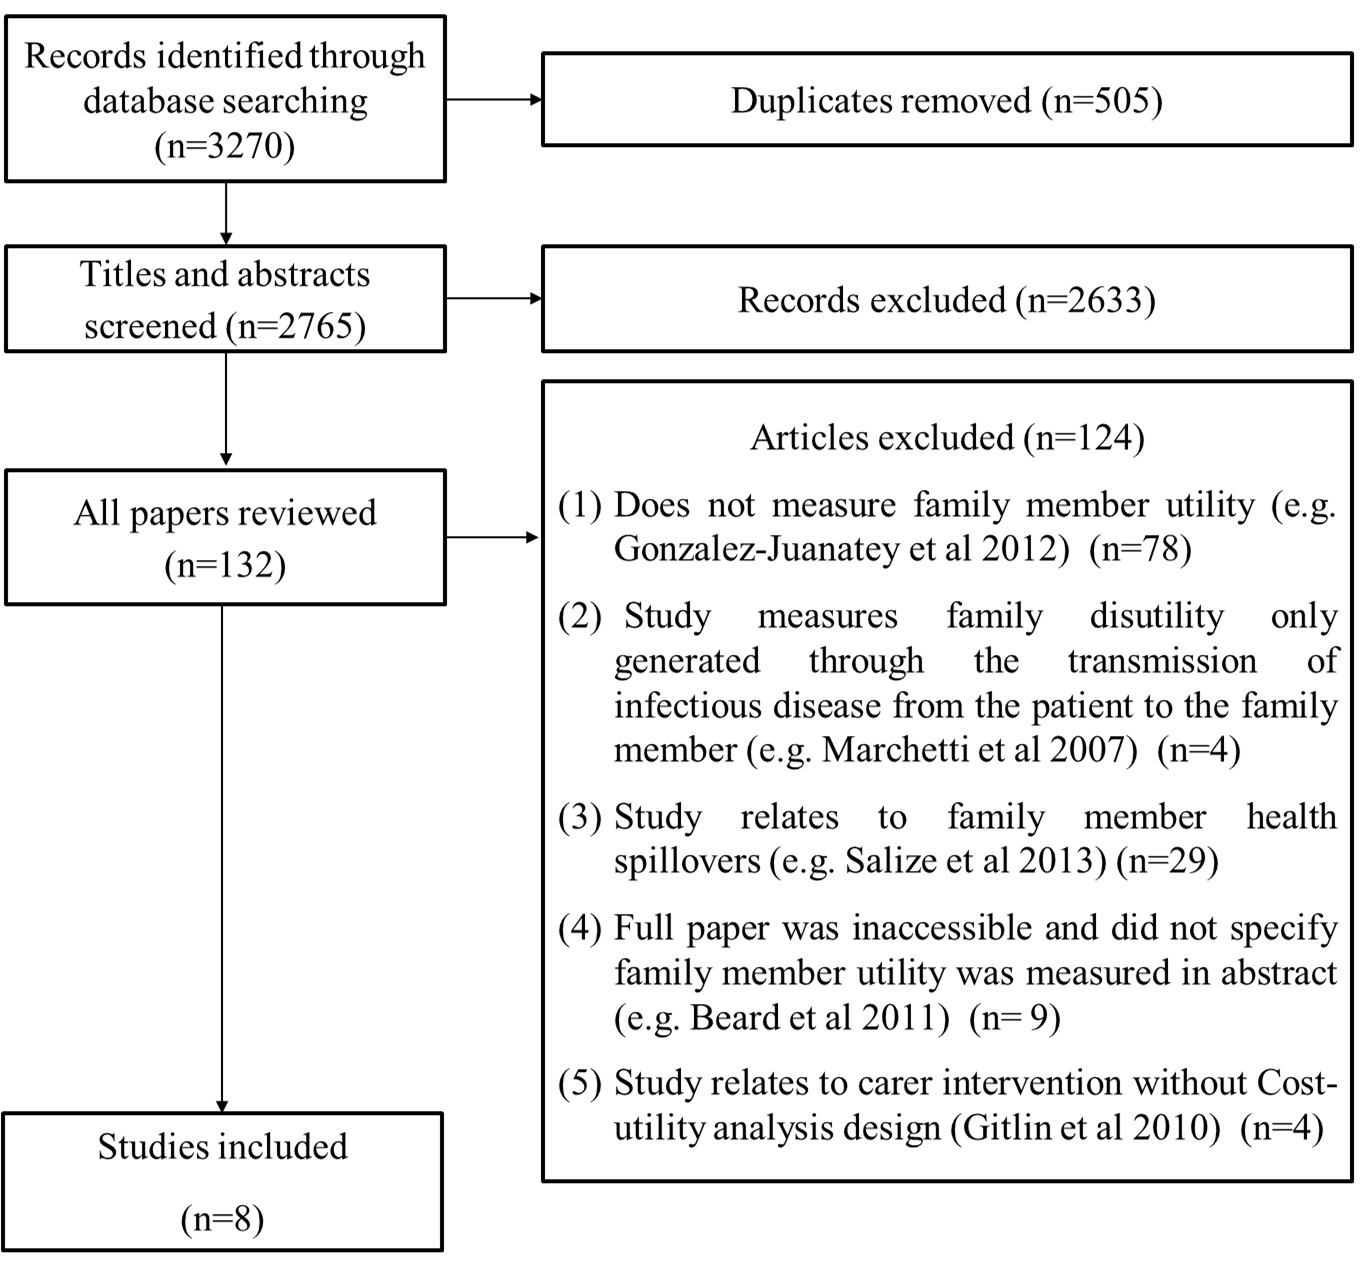
\includegraphics[width=1.0\linewidth]{prisma2.png}
\vspace{-0.1cm}
\caption{PRISMA flow diagram}
\end{figure}

\vspace{-1.0cm}
%\begin{enumerate}
\item Studies characteristics (N=8)
    \begin{itemize}
    \item \justifying Main Geographic area UK (N=5)
    \item Clinical fields: mental and/or behavioural (N=7) and cardiovascular (N=1)
    \item  Underpinning condition: Dementia (N=6), Stroke (N=1), Alzheimer (N=1)
    \end{itemize}
\end{enumerate}

\vspace{-1.7cm}
\begin{center}
%\begin{tabular}{ccc}

\includegraphics[width=2\linewidth]{logo3.png}
%\end{tabular}
\end{center}
%----------------------------------------------------------------------------------------


\end{block}

%----------------------------------------------------------------------------------------

\end{column} % End of column 2.2

\end{columns} % End of the split of column 2

\end{column} % End of the second column

\begin{column}{\sepwid}\end{column} % Empty spacer column

\begin{column}{\onecolwid} % The third column
%\vspace{-1.7cm}

%----------------------------------------------------------------------------------------

\begin{block}{}
%\vspace{-1.cm}
\begin{itemize}
     \item \justifying Cost-utility analyses: mainly based on randomized clinical trials (N=5)
    \item A Markov model based economic evaluation (N=1)
    \item Based on the cost and the effectiveness (ICER) results, the majority of the study (N=5) concluded the intervention to be effective, whereas N=2 studies  found interventions not effective. When going beyond the patient and/or caregiver case and targeting caregiver only, the findings were mitigated.
\end{itemize}
\vspace{-1.0cm}
\begin{enumerate}
    \item Critical review
\end{enumerate}
\vspace{-1.0cm}
\begin{figure}
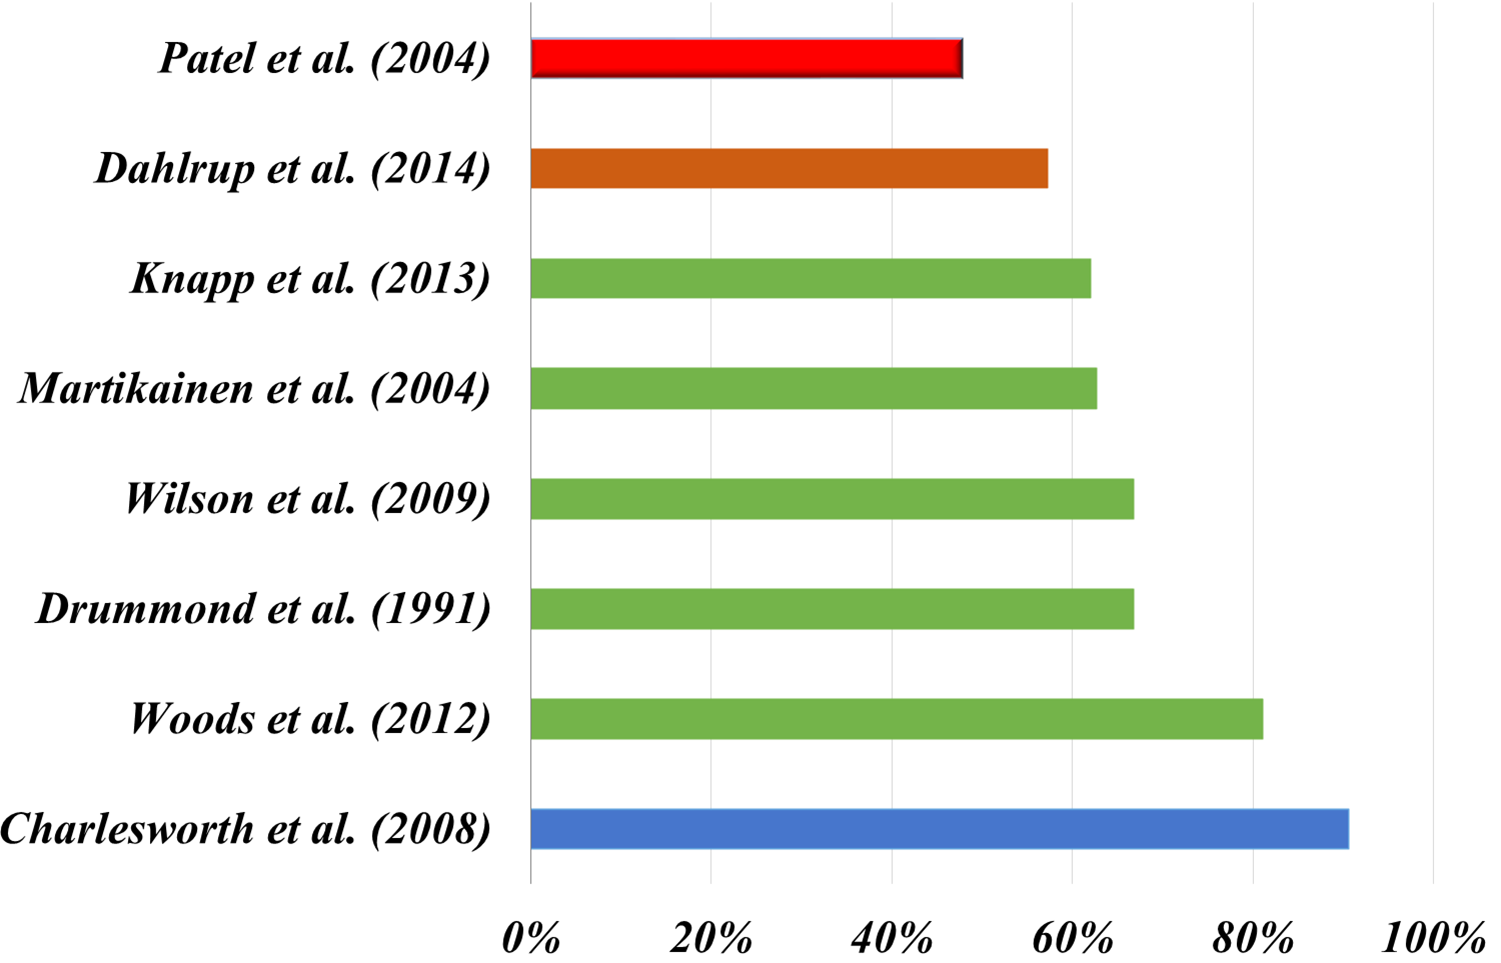
\includegraphics[width=1.0\linewidth]{stat_desc2.png}
\vspace{-0.5cm}
\caption{CHEERS score by studies}
\end{figure}

\end{block}


%----------------------------------------------------------------------------------------
%	IMPORTANT RESULT
%----------------------------------------------------------------------------------------
\vspace{-1.0cm}
\begin{alertblock}{Main Result}

\begin{itemize}
\item \justifying Seven of eight studies exceeded the 50\% CHEERS threshold.
\item Only one economic evaluation (Charlesworth et al., 2008) met the 85\% CHEERS score.
\end{itemize}

\end{alertblock} 
%----------------------------------------------------------------------------------------
%	CONCLUSION
%----------------------------------------------------------------------------------------
\vspace{-1.0cm}
\begin{block}{Conclusion}
\vspace{-0.5cm}
\begin{itemize}
    \item \justifying Our critical review highlights the lack of cost-utility analyses dealing with interventions to support informal caregivers and the relative paucity of good reporting practices. 
    \item Divergences in findings noticed across studies cannot be attributable only to difference in intervention undertake, but also on the scientific thoroughness.
   \end{itemize}
\end{block}
%----------------------------------------------------------------------------------------
%	ACKNOWLEDGEMENTS
%----------------------------------------------------------------------------------------

\setbeamercolor{block title}{fg=red,bg=white} % Change the block title color

%\begin{block}{Acknowledgements}
\vspace{-1.0cm}
\scriptsize \justifying \textbf{Acknowledgements:} This research was supported by the “Caisse Nationale de Solidarité pour l'Autonomie”, project “PERRIER-AAP16-Hand7-25” through the call for proposals launched by the IRESP in 2016.\\
%\begin{block}{Additional Information}
%\vspace{-1.1cm}
\scriptsize \justifying \textbf{Competing interests:} Travel, accommodation and conference registration of the presenter were supported by the Fondation MSD Avenir.

%\end{block}

%\end{block}

%----------------------------------------------------------------------------------------
%	CONTACT INFORMATION
%----------------------------------------------------------------------------------------

\setbeamercolor{block alerted title}{fg=black,bg=norange} % Change the alert block title colors
\setbeamercolor{block alerted body}{fg=black,bg=white} % Change the alert block body colors
\begin{alertblock}{Contact Information}
\begin{itemize}
\item \small Web: \href{https://www.gate.cnrs.fr/spip.php?article1124&lang=fr}{https://www.gate.cnrs.fr}
\item \small Email: \href{mailto: guets@gate.cnrs.fr}{ guets@gate.cnrs.fr}; \small Phone: +33 7 52 74 25 51
\end{itemize}
\end{alertblock}

%\vspace{-1.2cm}
----------------------------
%	REFERENCES
%----------------------------------------------------------------------------------------
\vspace{-1.0cm}
\begin{block}{References}
\vspace{-0.2cm}
\nocite{}{\scriptsize [1] Charlesworth, G., Shepstone, L., Wilson, E., Thalanany, M., Mugford, M., Poland, F., 2008. Does befriending by trained lay workers improve psychological well-being and quality of life for carers of people with dementia, and at what a cost? A randomised controlled trial. Health Technol. Assess.} \\
\nocite{}{\scriptsize [2] Dahlrup, B., Nordell, E., Steen Carlsson, K., Elmståhl, S., 2014. Health economic analysis on a psychosocial intervention for family caregivers of persons with dementia. Dement. Geriatr. Cogn. Disord. 37.}\\
\nocite{}{\scriptsize [3] Drummond, M.F., Mohide, E.A., Tew, M., Streiner, D.L., Pringle, D.M., Gilbert, J.R., 1991. Economic evaluation of a support program for caregivers of demented elderly. Int. J. Technol. Assess. Health Care 7.}\\
\nocite{}{\scriptsize [4] Knapp, M., King, D., Romeo, R., Schehl, B., Barber, J., Griffin, M., Rapaport, P., Livingston, D., Mummery, C., Walker, Z., Hoe, J., Sampson, E.L., Cooper, C., Livingston, G., 2013. Cost effectiveness of a manual based coping strategy programme in promoting the mental health of family carers of people with dementia (the START (STrAtegies for RelaTives) study): a pragmatic randomised controlled trial. BMJ 347. }\\
\nocite{}{\scriptsize [5] Martikainen, J., Valtonen, H., Pirttilä, T., 2004. Potential cost-effectiveness of a family-based program in mild Alzheimer’s disease patients. Eur. J. Heal. Econ. 5, 136–142.}
\nocite{}{\scriptsize [6] Patel, A., Knapp, M., Evans, A., Perez, I., Kalra, L., 2004. Training care givers of stroke patients : economic evaluation 328, 1–6}.\\
\nocite{}{\scriptsize [7] Wilson, E., Thalanany, M., Shepstone, L., Charlesworth, G., Poland, F., Harvey, I., Price, D., Reynolds, S., Mugford, M., 2009. Befriending carers of people with dementia: A cost utility analysis. Int. J. Geriatr. Psychiatry 24, 610–623.}\\
\nocite{}{\scriptsize [8] Woods, R., Bruce, E., Edwards, R., Elvish, R., Hoare, Z., Hounsome, B., Keady, J., Moniz-Cook, E., Orgeta, V., Orrell, M., Rees, J., Russell, I., 2012. REMCARE: reminiscence groups for people with dementia and their family caregivers – effectiveness and cost-effectiveness pragmatic multicentre randomised trial. Health Technol. Assess. (Rockv). 16.}\\
%Insert publications even if they are not cited in the poster
%\small{\bibliographystyle{unsrt}
%\bibliography{sample}\vspace{0.75in}}
\end{block}

%\vspace{-1.0cm}

%\begin{center}
%\begin{tabular}{ccc}
%
\includegraphics[width=1.0\linewidth]{logo3.png} %& \hfill & %
\includegraphics[width=0.4\linewidth]{logo2.png}
%\end{tabular}
%\end{center}

\vspace{-0.5cm}

\begin{center}
\textbf{ISPOR Europe 2018 | 10 -- 14 November 2018 | Barcelona, Spain. POSTER Code: PMH41 -- Date: 12/11/2018}
\end{center}
%----------------------------------------------------------------------------------------

\end{column} % End of the third column

\end{columns} % End of all the columns in the poster

\end{frame} % End of the enclosing frame

\end{document}
